\documentclass[11pt]{article}

\newcommand{\numpy}{{\tt numpy}}    % tt font for numpy

% for symbols
\usepackage{bbold}
\usepackage{amsmath,amssymb}
\DeclareMathOperator*{\argmin}{arg\,min}
\DeclareMathOperator*{\argmax}{arg\,max}
\setlength\parindent{20pt}

% for images
\usepackage{graphicx}
% \graphicspath{ {./images/} }


\DeclareRobustCommand{\bbone}{\text{\usefont{U}{bbold}{m}{n}1}}
\DeclareMathOperator{\EX}{\mathbb{E}}% expected value

\topmargin -.5in
\textheight 9in
\oddsidemargin -.25in
\evensidemargin -.25in
\textwidth 7in

\begin{document}

% ========== Edit your name here
\author{Monika, Jordi and Sebastian}
\title{Stochastic Modelling and Optimisation - Final Project}
\maketitle

\medskip

% ========== Begin answering questions here
\section{Motivation}
Nobody likes traffic. Traffic decreases the productivity of urban spaces, and translates into lower prosperity. Controlling the amount of traffic is therefore a priority goal for urban planners. Yet, most cities face natural or financial constraints in the expansion of transport networks. Consequently,  urban planners are faced with the challenge of optimising traffic flows within the constraints of existing infrastructure, to achieve the most efficient use of it possible.

In this project we study how dynamic programming can be applied to optimise urban traffic flows. Specifically, we study the traffic response urban control (TUC) strategy initially proposed by Diakaki, Papageorgiou, \& McLean (1999) to control traffic light signals.This strategy is based on a linear dynamic equation describing the number of cars present in a set of traffic link and a quadratic cost function, penalising the number of cars per link. This linear-quadratic system can be solved using infinite horizon dynamic programming. The strategy proceeds in two steps. First, a stationary policy prescribing green times to be used for any given state is computed off-line, using a set of parameters that describe the transport system, such as road capacity, cycle time, saturation flows and turning rates. Second, the dynamic policy responses are calculated for dynamically evolvoing state in a constrained minimisation problem, which ensures that the solution lies within a specified range of feasible green times, yet as close as possible to the optimal green times calculated in the first step. 

The solution the strategy provides is not globally optimal, because constraints are applied only after solving for the optimal policy matrix. However, breaking up the problem in these two steps has the practical advantage that the dynamic system can be solved 'off-line' and does not need to be continuously re-evaluated. Minimising deviation from the 'ideal policy' is then trivial and can be decentralised (to a traffic light control), which makes it easier to apply the system in real time and in large networks. The strategy nonetheless yields a solution that is forward-looking in the sense that any policy takes into account the effect of a change in a particular part of the system on the rest of the system (Diakaki, Papageorgiou, \& Aboudolas, 2001).

We simulate this strategy using a simple toy network of three junctions, connected by two main links, one of which is an 'upstream' link and one a 'downstream' link. The traffic flows only in one direction, from the upstream to the downstream link. We study how the strategy sets green times at the three junctions, and how it balances the benefit of allowing long green times to empty the upstream link with the resulting cost of potential downstream accumulation of cars. To gain a full understanding of the system dynamics, we vary parameters describing the infrastructure situation, such as road capacity, cycle time, saturation flow rates and turning rates and study the effect on the optimal green times chosen by the strategy.


We find that the transport network under our specification has [EXPAND with results, short preview of conclusion]

\section{DP formulation}
A transport network can be described as a set of links or approaches that connect a set of junctions. With respect to a junction, a link can be inflowing or outflowing, or both. The cycle time describes how long a full cycle of light changes takes at a given junction. Similarly, the total lost time describes how much of the cycle time is lost time, for example because all lights are red to allow pedestrians to pass. The number of stages divides the cycle time into a set of intervals during which a particular combination of links has right of way (r.o.w). The turning rates indicate the direction cars are turning into; they can be assumed to be an empirically established average. Saturation flows describe the capacity of a link; they can be assumed to be the maximum number of cars to pass the link during one control interval. The control interval can be set by the system administrator; it has to be at least as long as the shortest cycle time. The control interval determines how frequently green-light policies can be changed. If this interval is very long, then the system will react poorly to changing traffic situations. Demand and exit flows indicate whether cars enter the system or exit the system. Last but not least, green light times describe the length of time a particular link's signals give r.ow. to a certain stage of the signal cycle. This is the policy variable in this problem. Section 2.1 provides the notation for the above described variables.

\subsection{Variable definitions}
\begin{tabular}{ l l c }
Links (approaches): & $z \in Z$  &\\
Junctions: & $j \in J$ &\\
Set of inflowing links: & $I_j$ &\\
Set of outflowing links: & $O_j$ &\\
Cycle time (We assume $C_j = C$ for all junctions) : & $C_j$ & \\
Total lost time: &$L_j$ &\\
Set of stages: & $F_j$ &\\
Set of stages where link z has r.o.w.: & $v_z$ &\\
Saturation flow for link z: & $S_z$ &\\
Turning rates for inflowing link z and outflowing link w: & $t_{z,w}$ &\\
Control interval: & $T$ &\\
Period intervals: & $[k T,(k+1) T]$ &\\
Demand flow: & $d_z$ &\\
Exit flow: & $ s_z $ &\\
Green time of stage i at junction j: & $g_{j,i}$ &\\
Number of cars in link z: & $x_{z}$ & \\
\end{tabular}
\subsection{Constraints and indentities}
Several constraints have to be introduced to define a sensible transport network. Green times have an upper and lower bound, and cycle times are the sum of all green times for all stages plus the lost time. Exit flows for a given link are the product of the number of cars flowing into a link, and the turning rates indicating turns leading out of the network. Inflows to a given link are the sum of outflows from other links directed into the given link. Outflows are assumed to always occur at the maximum rate possible, whenever the respective stage has r.o.w.. If a given cycle includes more than one stage with r.o.w. for a given link, the sum of all green times for a given link are added to obtain the effective green time per cycle, which can in turn be used to calculate the average outflow from a given link per cycle. A steady state situation for a particular link is obtained when the outflows from the network equal the inflows plus the additional demand arising within the link (this can for example be parked cars entering the link, rather than cars entering from an inflowing link).

\begin{tabular}{ l l }
Green light constraints: & $g_{j,i} \in \left[g_{j, i, \min }, g_{j, i, \max }\right]$ \\
Cycle time constraint: & $\sum_{i \in F_{j}} g_{j, i}+L_{j}=C_j$ \\
Exit flow constraint: & $s_{z}(k)=t_{z, 0} q_{z}(k)$ \\
Inflow to link z: & $q_{z}(k)= \sum_{w \in I_{M}} t_{w, z} u_{w}(k)$ \\
Outflow from link z: & $u_z = \left\{ \begin{array} { l l } { S_z } & { \text { if  has r.o.w}  } \\ { 0 } & { \text { otherwise} } \end{array} \right.$ \\
(Assuming space available in downstream link and $x_z>S_z$)\\
Average value for outflow from z: & $u_{z}(k)=S_{z} G_{z}(k) / C$\\
Effective green time: & $G_{z}(k)=\sum_{i \in v} g_{j, i}(k)$ \\
Steady state demand: & $\left(1-t_{z, 0}\right) q_{z}^{N}+d_{z}^{N}-u_{z}^{N}=0$ \\
(Assuming nominal green times that lead to steady-state \\
link queues under non-saturating constant nominal demand) \\
\end{tabular}


\subsection{DP equations}
The number of cars in a given link z at the end of any given period k is the sum of the number of cars that remained in the link from the previous period, plus the cars that enter minus the cars that exit during the period. This yields the following dynamic equation:
\subsubsection*{Dynamics:}
\begin{equation}
x_{z}(k+1)=x_{z}(k)+T\left[q_{z}(k)-s_{z}(k)+d_{z}(k)-u_{z}(k)\right]
\end{equation}
Substituting gives:
\begin{equation}
x_{z}(k+1) =x_{z}(k)+T\left[\left(1-t_{z, 0}\right) \sum_{w \in I_{M}} \frac{t_{w, z} S_{w}\left(\sum_{i \in v_{w}} \Delta g_{M, i}(k)\right)}{C} +\Delta d_{z}(k)-\frac{S_{z}\left(\sum_{i \in v_{z}} \Delta g_{N, i}(k)\right)}{C} \right]
\end{equation}
In vector notation: 
\begin{equation}
\mathbf{x}(k+1)=\mathbf{A} \mathbf{x}(k)+\mathbf{B} \Delta \mathbf{g}(k)+\mathbf{T} \Delta \mathbf{d}(k)
\end{equation}

where $ \mathbf{x} $ is the state vector of the numbers of vehicles $ \mathbf{x}_z$ within links $z \in Z$ and $\Delta g_{j, i}=g_{j, i}-g_{j, i}^{\mathrm{N}}$ is a vector of deviations from steady-state green times and $\Delta d_{z}=d_{z}-d_{z}^{\mathrm{N}}$ is the deviation from the steady-state demand flows. $\mathbf{A}= \mathbf{I}$, $\mathbf{B}$ and  $\mathbf{T}$ are the state, input, and disturbance matrices, respectively. The input matrix B reflects the specific network topology, fixed staging, cycle, saturation flows, and turning rates. To solve the system we assume demand is in its steady-state: $\Delta \mathrm{d}(k)=0$.

\subsubsection*{Cost:}
To achieve the goal of minimising traffic accumulation in all links in the network, the number of cars in any given link is penalised quadratically. This introduces an automatic trade-off between links, as reducing the number of cars in one link leads to a higher number of cars in another link. This trade-off ensures that traffic is evenly distributed and no bottlenecks are created. Furthermore, deviations from the level of steady state green times are penalized quadratically. This ensures the system returns to a sensible equilibrium steady-state when green times are changed in a given period.
\begin{equation}
\mathcal{J}=\frac{1}{2} \sum_{k=0}^{\infty}\left(\|\mathbf{x}(k)\|_{\mathbf{Q}}^{2}+\|\Delta \mathbf{g}(k)\|_{\mathbf{R}}^{2}\right)
\end{equation}

$\mathbf{Q}$ and $\mathbf{R}$ in the cost equation are non-negative definite, diagonal weighting matrices. Since the first term in (4), $\|\mathbf{x}(k)\|_{\mathbf{Q}}^{2}$ is responsible for minimisation and balancing of the relative occupancies of the network links, $\mathbf{Q}$ has its diagonal elements equal to the inverses of the storage capacities of the corresponding links. $\mathbf{R}$ influences the magnitude of the control reactions.  $\mathbf{R}=r\mathbf{I}$, where the choice of r is picked to ensure the best results for a given application network (i.e. simple trial-error procedure). Both matrices can be modified in case any particular link carries increased significance. The infinite sum in the cost equation (4) suggest an infinite time horizon, which is used in order to obtain a time-invariant feedback law according to LQ optimisation theory. 

\subsubsection*{Solution of the DP Problem:}
To minimise the cost presented in equation (4) subject to the dynamics in (3), we follow Bertsekas (2005, Vol 2., pp.140). The problem is a discrete-time linear quadratic control problem with infinite-horizon, which is solved via the algebraic Riccati equation. 

We define a symmetric positive definite \textbf{cost-to-go matrix $K$} evolving backwards in time from $K _ { N } = Q$ according to:
\begin{equation} 
K _ { k - 1 } = Q + A ^ { T } K_ { k } A - A ^ { T } K _ { k } B \left( B ^ { T } K_ { k } B + R \right) ^ { - 1 } B ^ { T } K _ { k } A
\end{equation}
This is the discrete-time dynamic Riccati equation of this problem. The steady-state characterization of $K$, relevant for the infinite-horizon problem in which $k$ goes to infinity, can be found by iterating the dynamic equation repeatedly until it converges; then $K$ is characterized by removing the time subscripts from the dynamic equation. Resulting in the algebraic Riccati equation of this problem:
\begin{equation}
K = Q+ A ^ { T } K A - \left( A ^ { T } K B \right) \left( R + B ^ { T } K B \right) ^ { - 1 } \left( B ^ { T } K A \right)
\end{equation}

The solution to this problem yields a stationary policy given by the control matrix $\mathbf{L}$:
\begin{equation}
\mathbf{L} = \left(B ^ { T } K B +R \right) ^ { - 1 } B ^ { T } K A 
\end{equation}

Putting it into DP framework that uses backwards induction, the optimal control solution at each time k is equivalent to:
\begin{equation} 
\Delta g _ { k } ^ { * } = - \left( B ^ { T } K _ { k } B + R \right) ^ { - 1 } \left( B ^ { T } K _ { k } A \right) x _ { k - 1 }
\end{equation}

Dropping the k's because of the infinite horizon assumption, the equation transforms to:

\begin{equation} 
\Delta g  ^ { * } = - \left( B ^ { T } K  B + R \right) ^ { - 1 } \left( B ^ { T } K  A \right) x _ { k - 1 }
\end{equation}

And can equivalently by written as:
\begin{equation} 
\mathbf { g } ( k ) = \mathbf { g } ^ { \mathrm { N } } - \mathbf { L } \mathbf { x } ( k )
\end{equation}
where $\Delta \mathbf {g } = \mathbf { g } ( k ) - \mathbf {g } ^ { \mathrm { N } }$.\\

In order to avoid computation of steady state green times, we take first differences of the control law:

\begin{equation} 
\mathbf { g } ( k ) = \mathbf { g } (k-1)  - \mathbf { L } [ \mathbf { x } ( k ) - \mathbf { x } ( k -1 )]
\end{equation}

The above derived green times may not lie within the feasible range defined in section 2.2, because the LQ problem presented above does not consider control constraints. Those, however, can be imposed after the solution to (10) is computed. Hence, this calls for another optimisation problem that is solved in real-time for each junction $j$ so as to specify feasible green times $G _ { j , i }$ that are closest in distance to the non-feasible regulator-based green times $g _ { j , i }$ resulting from (10).

\begin{equation} \operatorname { min } { G _ { j , i } } \sum _ { i \in F _ { j } } \left( g _ { j , i } - G _ { j , i } \right) ^ { 2 }\end{equation} 
subject to
\begin{equation} 
\sum _ { i \in F _ { j } } G _ { j , i } + \left| L _ { j } = C \right.
\end{equation} 
\begin{equation} 
G _ { j , i } \in \left[ g _ { j , i , \min } , g _ { j , i , \max } \right] \forall i \in F _ { j }
\end{equation} 

\section{Simulations}
To understand the workings of the TUC strategy, we apply it to a simple toy network of three junctions (O,M,N - depicted in figure 1). The network further consists of two connecting links (A,B) and 5 traffic lights that will be used to control the traffic flow. Two links flow into the network at junction M (w1, w2) and one link flows into the network at junction B (w3). Traffic in this network is one-way, there is no traffic from O to M. All traffic flows considered are marked by red arrows, and traffic lights are marked by a black barrier in the road. 


Find below the dynamic equations of the toy network explaine above and that will help to understand below results.

\begin{equation}
x_{A}(k+1)=x_{A}(k)+T\left[\left(1-t_{A,0}\right)\bigg[\frac{t_{w_{1},A}S_{w_{1}}\Delta g_{M,1}(k)}{C}+\frac{t_{w_{2},A}S_{w_{2}}\Delta g_{M,2}(k)}{C}\bigg]+\Delta d_{A}(k)-\frac{S_{A}\Delta g_{N,1}(k)}{C}\right]
\end{equation}

\begin{equation}
x_{B}(k+1)=x_{B}(k)+T\left[\left(1-t_{B,0}\right)\bigg[\frac{t_{A,B}S_{A}\Delta g_{N,1}(k)}{C}+\frac{t_{w_{3},B}S_{w_{3}}\Delta g_{N,2}(k)}{C}\bigg]+\Delta d_{B}(k)-\frac{S_{B}\Delta g_{0,1}(k)}{C}\right]
\end{equation}


The toy network we study is the simplest possible network to sensibly apply the TUC strategy. The strategy requires at least two connecting links to show its dynamics, as it can then balance traffic across the two links. Of course the advantages of the TUC strategy mostly lie in the regulation of large networks with saturated traffic flows. Given the simplicity of the toy network we study, other solutions to achieve optimal control can be used to find a true global optimum. However, in this project we aim to understand the mechanics of the TUC strategy rather than test its performance, which is why we choose this rather minimalistic setup. We refer the interested reader to Diakaki, Papageorgiou, \& Aboudolas (2001) for an evaluation of the strategy's performance.

In this section we will assess how the network reacts to a perturbation (increase in the demand / number of cars that join the two links of the network in a given control period), and how this reaction differs depending on the parameterisation of the network. The two parameters we study are:

\begin{itemize}
\item Turning rate from A to B ($t_{AB}$) - higher proportion of cars from link A continues to link B
\item Saturation flow of the lateral roads ($S_{w2,A}$ and $S_{w3,B}$) - more cars from the lateral connection can enter during a control cycle
\item \% of cars leaving the network at each link ($t_0$) - cars entering the parking garage
\end{itemize}


\begin{figure}[h!]
    \caption{Network Graph}
      \centering
	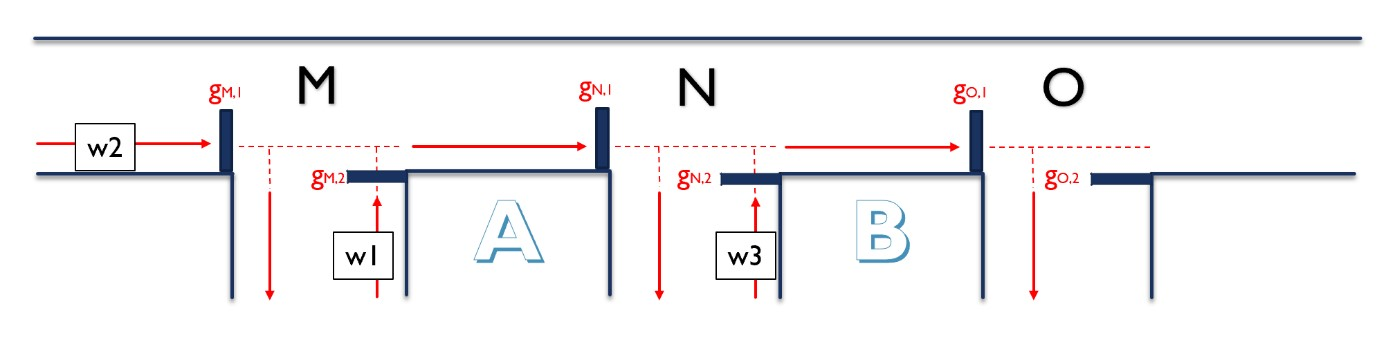
\includegraphics[width=18cm]{network-graph}
\end{figure}

\subsection{Results}

The results will be presented in panels of two figures: on the left, we see the evolution of the number of cars in the link at each period as a consequence of a perturbation. This perturbation is an increase in demand $d$ that gets added to every link. We like to think of this as cars entering the links from a parking garage. 
On the right we see the green times of the different signals evolving over the periods as a consequence of the TUC strategy imposed to the network. Therefore, the traffic lights react to the number of cars that are stopped in the link. In our base scenario, we assume that 50\% of cars in link A turn to link B, and that the saturation flow/ the number of cars entering each link from the lateral inflows is 40 per control cycle, and that 30\% of cars in every link reach their destination in the link (they exit the network). Initially, the green times are all set to 50 seconds, and all links are empty. Figure 2 depicts this base case scenario over 100 periods, with demand perturbations until period 50. We see that both links become saturated in the first 10 periods, and remain saturated until the demand perturbations subside. Link A remains saturated longer than link B, which is to be expected because link A can only be emptied when the downstream link B has free capacity. As few cars as possible are let pass from link A to link B while link B is still saturated, as can be seen in the green light times for $G_{N1}$. The green light times for  $G_{N1}$ and  $G_{N2}$ are reciprocal, as are the green light times for $G_{M1}$ and  $G_{M2}$. 

\begin{figure}[h!]
    \caption{Base scenario - Medium turning rate, saturation flow, and outflow}
      \centering
	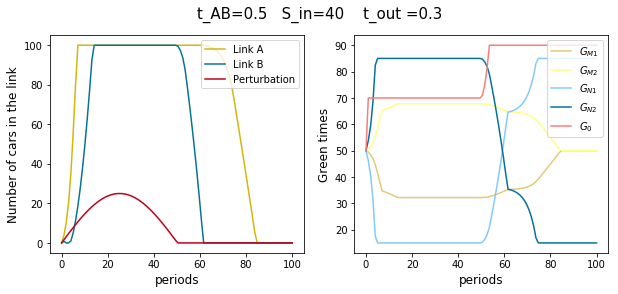
\includegraphics[width=13cm]{sim4}
\end{figure}

\subsubsection{Turning rate AB}


Increasing the turning rate from A to B is equivalent to increasing the percentage of cars that flow from link A to link B, rather than turning right and exiting the network. The evolution of the system at turning rates of 20 and 30\% is shown in figures 3 and 4.

Note that the lower the turning rate, the lower the number of cars in link A waiting to pass to B. In the case of a low turning rate, emptying link A with longer green times for $G_{N1}$ therefore is 'easier' and begins sooner after the perturbation. At very high turning rates link A always remains oversaturated. % add why

\begin{figure}[h!]
    \caption{Low turning rate}
      \centering
	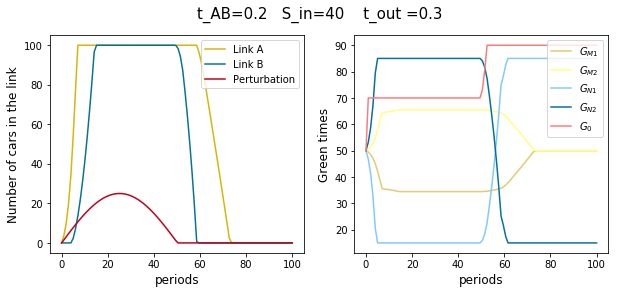
\includegraphics[width=13cm]{sim1}
\end{figure}

\begin{figure}[h!]
    \caption{High turning rate}
      \centering
	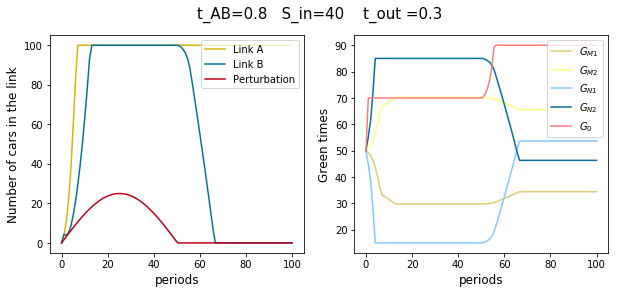
\includegraphics[width=13cm]{sim8}
\end{figure}


\subsubsection{Saturation inflow}

Modifying the saturation flow is equivalent to changing the number of cars that enter the network from the lateral roads. In reality this can be achieved, for example, by reducing the number of lanes. The results of low and high saturation flows are shown in figure 5 and 6.

We can clearly see that when the saturation coefficient goes beyond 50, both links are completely congested. The r.o.w times of the lateral roads increase until their feasible maximum in order to allow as many as possible lateral inflowing cars in.

\begin{figure}[h!]
    \caption{Low saturation flow}
      \centering
	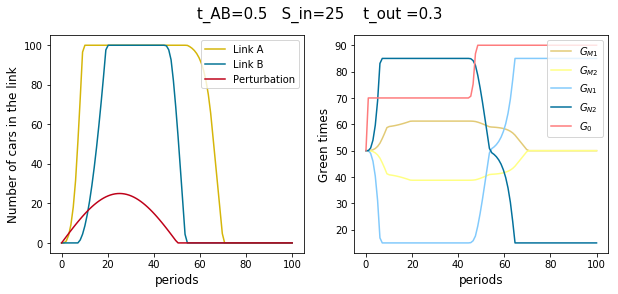
\includegraphics[width=13cm]{sim2}
\end{figure}

\begin{figure}[h!]

    \caption{High saturation flow}
      \centering
	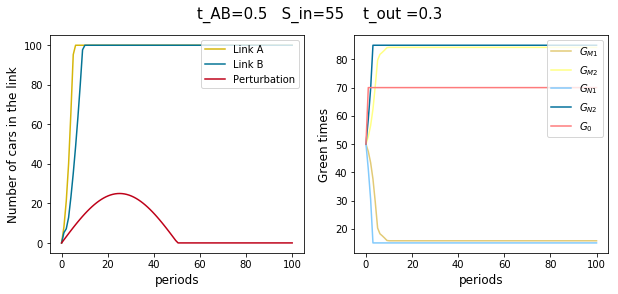
\includegraphics[width=13cm]{sim7}
\end{figure}

\subsubsection{Outflowing traffic}

In this subsection we assess the effect of letting more cars out the system from the lateral roads. Logically, the more cars leave the network, the emptier the links are. The results of low and high outflow are shown in figure 7 and 8.

Note that if the total amount of cars leaving the system is less than 10\% the network gets congested and, similarly to what we have seen in previous cases, the r.o.w times do not fluctuate.

\begin{figure}[h!]
    \caption{Low outlfow}
      \centering
	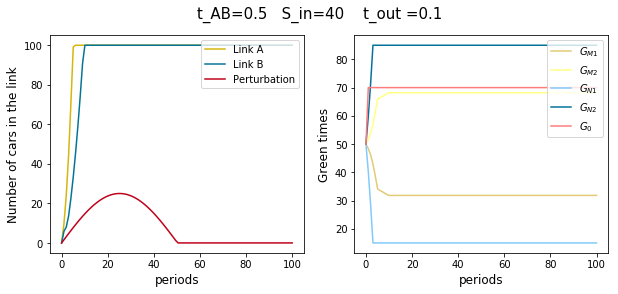
\includegraphics[width=13cm]{sim3}
\end{figure}

\begin{figure}[h!]
    \caption{High outflow}
      \centering
	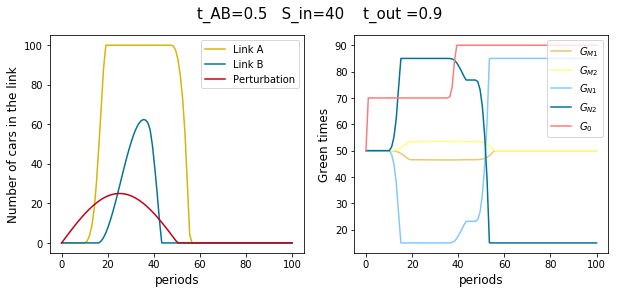
\includegraphics[width=13cm]{sim6}
\end{figure}

\subsubsection{Comparison varying vs fixed r.o.w times}

One may wonder if varying r.o.w time as a function of the link occupancy really improves network efficiency. To check that, we compared the performance of the network by applying a variable r.o.w time (TUC) and a fixed time policy. 

Figure 9 shows the differences in number of cars for each period for both policies. In effect, the TUC strategy is more efficient than setting the lights to a fixed time. Whereas time varying policy succeeds to empty the link A before the 100th period, the fixed policy struggles to empty it and after period 100 the link is still congested.

\begin{figure}[h!]
    \caption{Variable vs. fixed green times}
      \centering
	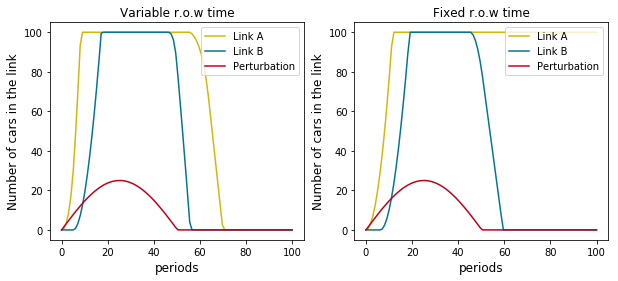
\includegraphics[width=12cm]{sim9}
\end{figure}

\section{Conclusions}

We conclude that the control matrix L derived in the TUC strategy provides a control law with a robust gating feature to protect down-stream links from oversaturation. Roughly speaking, the higher the number of vehicles within a particular link the lower the green times of the links that lead into it are set. It is important to notice, as seen in all the simulations, that the regulator has a reactive rather than anticipatory behaviour where it responds indirectly to unknown disturbances, and therefore, it cannot make use of predictions of the future traffic conditions. 
 \clearpage

\begin{thebibliography}{9}
\bibitem{bertsekas} 
Bertsekas, D. (2005). Dynamic Programming and Optimal Control (3rd ed.). Athena Scientific.

\bibitem{diakaki1} 
Diakaki, C., Papageorgiou, M. \& Aboudolas, K. (2001).
A multivariable regulator approach to traffic-responsive network-wide signal control.
\textit{Control Engineering Practice} 10, 183-195.

\bibitem{diakaki2} 
Diakaki, C., Papageorgiou, M., \& McLean, T. (1997). Simulation studies of integrated corridor control in Glasgow. 
\textit{Transportation Research C}, 5, 211-224.

\end{thebibliography}

% ========== Continue adding items as needed

\end{document}
\grid
\grid